\documentclass{article}

\usepackage{tikz}
\usetikzlibrary{arrows.meta}

% ---------- Colors ----------
\definecolor{navy}{RGB}{20,55,100}
\definecolor{steel}{RGB}{70,100,130}
\definecolor{gold}{RGB}{190,140,40}
\definecolor{goldpale}{RGB}{255,248,220}
\definecolor{bluepale}{RGB}{235,242,250}

\begin{document}
	
	\begin{figure}[ht]
		\centering
		
		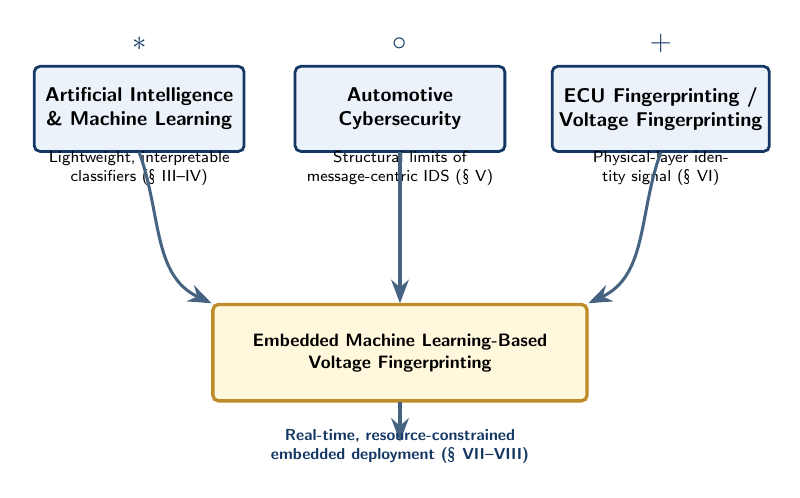
\begin{tikzpicture}[scale=0.72, transform shape]
			
			% ==================================================
			% TOP THREE BLOCKS
			% ==================================================
			
			\node[
			rectangle,
			rounded corners=2pt,
			draw=navy,
			fill=bluepale,
			line width=1pt,
			minimum width=3.7cm,
			minimum height=1.5cm,
			align=center,
			font=\sffamily\bfseries
			] (s1) at (0,4.6)
			{\textbf{Artificial Intelligence}\\
				\textbf{\& Machine Learning}};
			
			\node[
			rectangle,
			rounded corners=2pt,
			draw=navy,
			fill=bluepale,
			line width=1pt,
			minimum width=3.7cm,
			minimum height=1.5cm,
			align=center,
			font=\sffamily\bfseries
			] (s2) at (4.6,4.6)
			{\textbf{Automotive}\\
				\textbf{Cybersecurity}};
			
			\node[
			rectangle,
			rounded corners=2pt,
			draw=navy,
			fill=bluepale,
			line width=1pt,
			minimum width=3.7cm,
			minimum height=1.5cm,
			align=center,
			font=\sffamily\bfseries
			] (s3) at (9.2,4.6)
			{\textbf{ECU Fingerprinting /}\\
				\textbf{Voltage Fingerprinting}};
			
			% ==================================================
			% SIMPLE ICONS
			% ==================================================
			
			\node[
			font=\Large\bfseries,
			text=navy
			] at (0,5.75) {$\ast$};
			
			\node[
			font=\Large\bfseries,
			text=navy
			] at (4.6,5.75) {$\circ$};
			
			\node[
			font=\Large\bfseries,
			text=navy
			] at (9.2,5.75) {$+$};
			
			% ==================================================
			% DESCRIPTIONS
			% ==================================================
			
			\node[
			font=\sffamily\footnotesize,
			text width=3.7cm,
			align=center
			] at (0,3.55)
			{Lightweight, interpretable classifiers
				(\S~III--IV)};
			
			\node[
			font=\sffamily\footnotesize,
			text width=3.7cm,
			align=center
			] at (4.6,3.55)
			{Structural limits of message-centric IDS
				(\S~V)};
			
			\node[
			font=\sffamily\footnotesize,
			text width=3.7cm,
			align=center
			] at (9.2,3.55)
			{Physical-layer identity signal
				(\S~VI)};
			
			% ==================================================
			% CENTRAL CONVERGENCE BLOCK
			% ==================================================
			
			\node[
			rectangle,
			rounded corners=2pt,
			draw=gold,
			fill=goldpale,
			line width=1.2pt,
			minimum width=6.6cm,
			minimum height=1.7cm,
			align=center,
			font=\sffamily\bfseries\small
			] (c) at (4.6,0.3)
			{Embedded Machine Learning-Based\\
				Voltage Fingerprinting};
			
			% ==================================================
			% ARROWS TO CENTRAL BLOCK
			% ==================================================
			
			\draw[
			-{Stealth[length=3mm]},
			line width=1.1pt,
			draw=steel
			] (s1.south) to[out=-70,in=155] (c.north west);
			
			\draw[
			-{Stealth[length=3mm]},
			line width=1.1pt,
			draw=steel
			] (s2.south) -- (c.north);
			
			\draw[
			-{Stealth[length=3mm]},
			line width=1.1pt,
			draw=steel
			] (s3.south) to[out=-110,in=25] (c.north east);
			
			% ==================================================
			% DOWNWARD ARROW
			% ==================================================
			
			\draw[
			-{Stealth[length=3mm]},
			line width=1.1pt,
			draw=steel
			] (c.south) -- ++(0,-0.7);
			
			% ==================================================
			% FINAL DESCRIPTION
			% ==================================================
			
			\node[
			font=\sffamily\bfseries\footnotesize,
			align=center,
			text=navy
			] at (4.6,-1.35)
			{Real-time, resource-constrained\\
				embedded deployment (\S~VII--VIII)};
			
		\end{tikzpicture}
		
		\caption{Convergence of AI/ML Progress, Automotive Cybersecurity, and ECU Fingerprinting Toward Embedded Voltage Fingerprinting.}
		
		\label{fig:convergence}
		
	\end{figure}
	
\end{document}